\begin{frame}
    \Huge
    \begin{center}
        \textbf{Conditional Probability}
    \end{center}
\end{frame}

\subsection{Definition}\label{subsec:definition2}
\begin{frame}
    \frametitle{Definition}
    \begin{block}{}
        In probability theory, conditional probability is a measure of the probability of an event occurring, given that another event (by assumption, presumption, assertion or evidence) has already occurred.
    \end{block}
\end{frame}

\subsection{Notations}\label{subsec:notations2}
\begin{frame}
    \frametitle{Notations}
    \begin{block}{}
        \begin{itemize}
            \item $P[A|B]$: Probability of $A$ given $B$.
            \item $P[A|B=b]$: Probability of $A$ given $B=b$.
        \end{itemize}
    \end{block}
\end{frame}

\subsection{Equation}\label{subsec:equation2}
\begin{frame}
    \frametitle{Equation}
    \begin{block}{}
        \begin{equation}
            P[A|B] = \frac{P[A \cap B]}{P[B]}\label{eq:equation21}
        \end{equation}
    \end{block}
\end{frame}

\subsection{Example}\label{subsec:example2}
\begin{frame}
    \frametitle{Example}
    For example, the probability that any given person has a cough on any given day may be only 5\%.
    But if we know or assume that the person is sick, then they are much more likely to be coughing.
    For example, the conditional probability that someone unwell (sick) is coughing might be 75\%, in which case we would have that $P(Cough) = 5\%$ and $P(Cough|Sick) = 75\%$.
\end{frame}

\subsection{Analysis}\label{subsec:analysis2}
\begin{frame}
    \frametitle{Analysis}
    The unconditional probability:
    \begin{itemize}
        \item $P(A) = 0.30 + 0.10 + 0.12 = 0.52$.
    \end{itemize}
    The conditional probability:
    \begin{itemize}
        \item $P(A|B1) = 1$.
        \item $P(A|B2) = 0.12 \div (0.12 + 0.04) = 0.75$
        \item $P(A|B3) = 0$.
    \end{itemize}
    \begin{figure}[h]
        \centering
        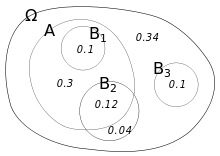
\includegraphics[width=0.4\linewidth]{./img/220px-Conditional_probability.svg}
        \caption{Illustration of conditional probabilities with an Euler diagram.}
        \label{fig:example2}
    \end{figure}
\end{frame}

\subsection{As an axiom of probability}\label{subsec:axiom}
\begin{frame}
    \frametitle{As an axiom of probability}
    Some authors, such as de Finetti, prefer to introduce conditional probability as an axiom of probability:
    \begin{block}{}
        \begin{equation}
            P(A \cap B) = P(A|B) \cdot P(B)\label{eq:equation22}
        \end{equation}
    \end{block}
    This equation for a conditional probability, although mathematically equivalent, may be intuitively easier to understand.
\end{frame}
